
\subsection{Экспериментальная часть}
Для экспериментальной оценки реализации предложенного решения мы использовали набор данных GTD\_0616 \cite{db:gtd}.
% GTD description
Этот набор данных обладает следующими особенностями:
	\begin{enumerate}
		\item Содержит подробную информацию о терактах начиная с 1975 года
		\item Содержит 55'600 записей с 1991 по 2012 год
        \item Информация включает в себя подробное описание теракта: дата, страна, группировка, ущерб, ...
        \item Содержит разнородные признаки: количественные, категориальные и, для некоторых событий, текстовые описания.
	\end{enumerate}

% Data aggregation using NMF model
\subsubsection{Построение представления событий и интерпретируемость}
Чтобы получить необходимое нам представление событий в пространстве тематик, были использованы алгоритм матричной факторизации NMF и нейросетевой подход, основанный на автокодировщиках.
После преобразований, описанных в начале раздела \ref{subsub:repr} и агрегирования мы перешли от отдельных событий к \textit{временному периоду}, содержащему некоторые события с помощью усреднения значений тематик для событий, входящих в этот период. Далее будем называть этот период \textit{агрегационным периодом} или просто \textit{периодом}. Затем к предобработанным данным мы применяли методы построения представления событий, пример 10 выделенных тематик как результат работы алгоритма неотрицательной факторизации матриц можно видеть на  Рис. \ref{fig:features_example}.

\begin{figure}
  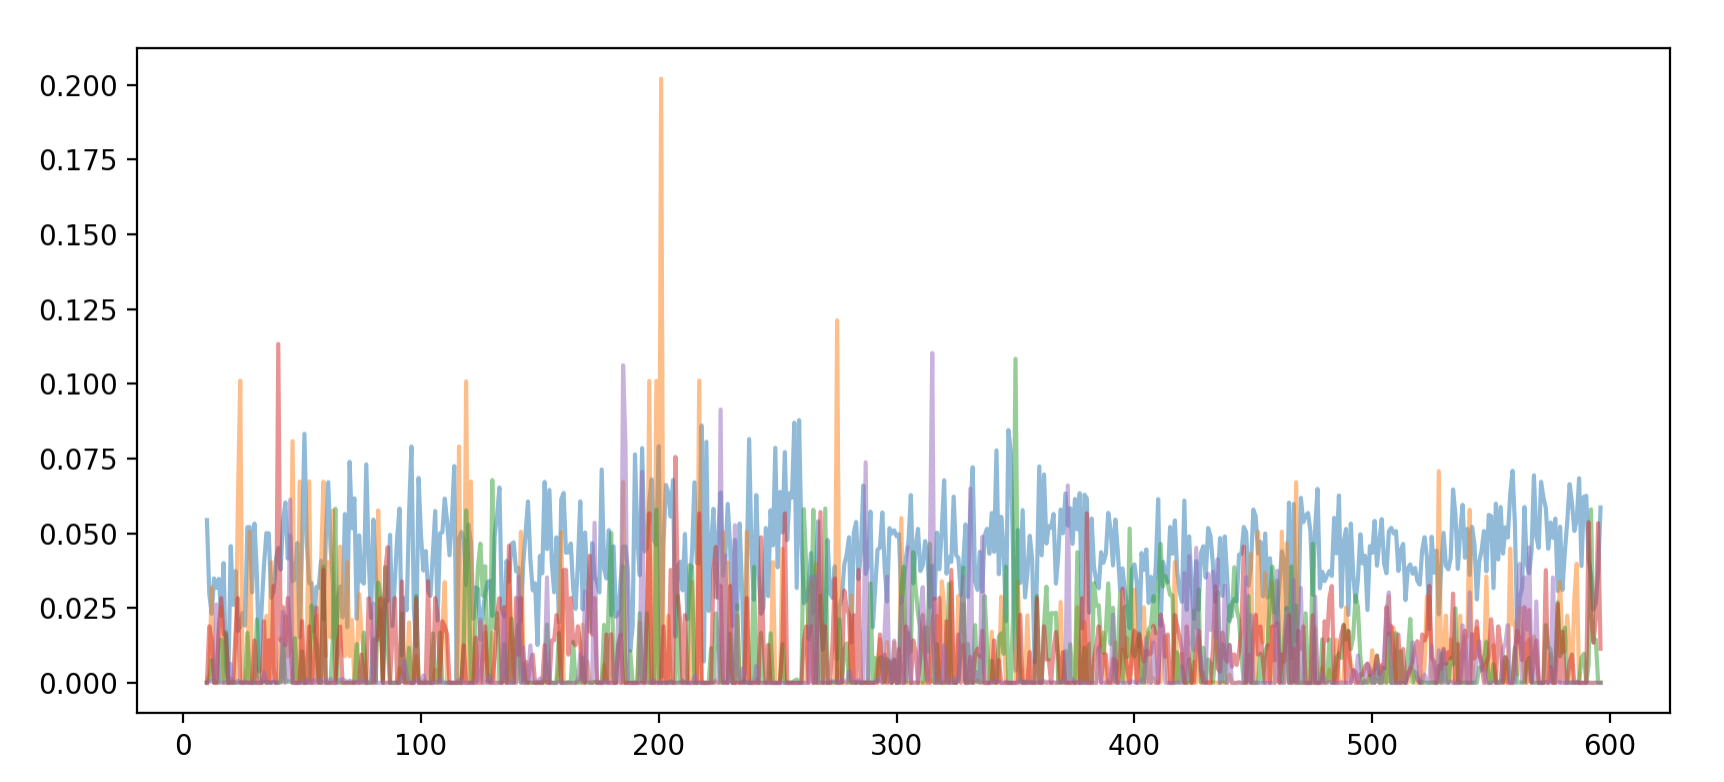
\includegraphics[width=\linewidth]{features_example.png}
  \caption{Пример временных рядов для тематик NMF}
  \label{fig:features_example}
\end{figure}

В случае с нейросетевым автокодировщиком, использовалась архитектура, описанная в таблице \ref{table:ae_arch}. Для кодировщика последовательно использовались полносвязные слои размерностей 256, 128 и 50 (размерность кода). Для декодировщика использовались полносвязные слои тех же размерностей, но в обратном порядке. Размерность входного вектора была равна 414, в рамках экспериментов были исследованы размерности скрытого кода равные 10 и 50. Для обучения модели применялась функция потерь $MAE$, описанная выше.
Количество эпох (т.е. количество проходов по всем имеющимся данным) при обучение модели было выбрано равным 100, начальный темп обучения был выбран равным  $2\cdot 10^{-3}$, также было использование экспоненциальное затухание темпа обучения: после каждой эпохи величина темпа обучения умножалась на 0.96.

\begin{table}
\centering
 \begin{tabular}{| c | c | c | c | c |} 
 \hline
 Название слоя & Тип слоя & Размер входа & Размер выхода & Функция активации\\
 \hline
 \hline
 кодировщик(1) & Полносвязный & 414 & 256 & ReLU\\ 
 \hline
 кодировщик(2) & Полносвязный & 256 & 128 & ReLU\\ 
 \hline
 кодировщик(3) & Полносвязный & 128 & 50 & ReLU\\ 
 \hline
 декодировщик(1) & Полносвязный & 50 & 128 & ReLU\\ 
 \hline
 декодировщик(2) & Полносвязный & 128 & 256 & ReLU\\ 
 \hline
 декодировщик(3) & Полносвязный & 256 & 414 & ReLU\\ 
 \hline
\end{tabular}
\caption{Архитектура автокодировщика}
\label{table:ae_arch}
\end{table}

Для интерпретации тематик методом, описанным в \ref{subsub:interp}, из набора данных были извлечены 19335 событий с текстовыми описаниями. После предобработки описаний и выделения слов был получен словарь размера 2311. После применения всей процедуры, описанной в \ref{subsub:interp} были получены наборы ключевых слов, описывающие тематики. Примеры таких ключевых слов для первых 5 тематик указаны в таблице \ref{table:kw_example}.

\begin{table}
\centering
 \begin{tabular}{c c} 
 \hline
 Тематика & Ключевые слова\\ 
 \hline
 \hline
 0 & used, sources, available, majority, listed, database, ...\\
 \hline
 1 & shot, civilian, distributed, bomb, detonated, ...\\
 \hline
 2 & taliban, shrine, perpetrators, tamil, rebels, group, ...\\
 \hline
 3 & released, hostage, kidnapping, status, abduction, ...\\
 \hline
 4 & indicated, military, police, civilian, detonating, ...\\
 \hline
 \end{tabular}
\caption{Примеры ключевых слов из описаний тематик }
\label{table:kw_example}
\end{table}


\subsubsection{Описание процесса обучения и тестирования} \label{train_process}
% NMF topics with lags as features
Метод прогнозирования, описываемый в моей работе, основывается на предположении, что вероятность наступления события (или количество событий) зависит от предшествующих событий, а точнее от значений тематик в агрегационных периодах, предшествующих периоду, для которого мы предсказываем эту вероятность.
В качестве признаков использовались значения тематик из $L$ предшествующих периодов, и таким образом для $k$ тематик размерность итогового пространства признаков становилась равна $L \cdot k$.

% target generation
Чтобы сформировать \textit{целевую переменную} необходимо было сначала определить события, которые нас интересуют (далее - \textit{целевые события}), в этой работе такие события определены как теракты, произошедшие в Ираке с типом атаки "взрыв". Затем каждому событию ставилась в соответствие метка: 1, если это интересующее нас событие и 0 иначе. 

% Далее, метка для агрегационного периода целиком ставилась в зависимости от решаемой задачи:
% \begin{enumerate}
%     \item Классификация:  1, если в период входит хотя бы одно событие с меткой 1, 0 иначе. Таким образом метка периода соответствует индикатору, произошло ли целевое событие в течение этого периода.
%     \item Регрессия: Сумма меток всех событий, входящих в период, целое неотрицательное число, представляет собой количество целевых событий, произошедших за этот период.
% \end{enumerate}

Поскольку данные имеют очевидную временную составляющую, то разбиение на \textit{тренировочную} и \textit{тестовую} выборку производилось строго последовательно: первые 70\% данных отводились для тренировочной выборки, а оставшиеся 30\% - для тестовой.

% Metrics: ROC AUC, MAE
Для оценки качества решения в задаче классификации использовалась метрика ROC AUC, как уже было сказано выше, одно из ее преимуществ заключается в том, что она инвариантна к несбалансированности классов (в отличие, например, от метрики "Точность"). Поскольку в задачах прогнозирования событий реальные данные редко бывают сбалансированы, применение этой метрики является более разумным выбором для отражения качества прогноза.

В задаче регрессии для оценки решения была выбрана метрика MASE, которая считается по формуле, описанной в \ref{sect:event_forecast}.

% \subsection{Выбор разбиения данных} 
% \textit{Разбиение данных} - набор величин (год начала, год конца, длина периода агрегации, размер тренировочной выборки и правила для выбора целевых событий), характеризующий данные, получаемые после агрегации и генерации целевой переменной.\par
% % Automated time period choosing, different stats calculations
% Выше были определены признаки, которые будут использоваться для решения поставленных задач, и была упомянута проблема несбалансированных данных.
% На самом деле, если взять произвольные правила для определения целевого события (напр: страна Пакистан, тип атаки: Похищение) может оказаться, что ни один агрегационный период не содержит таких событий. Решение таких задач относится к области "прогнозирование экстремально редких событий (extreme rare event prediction) и выходит за рамки этой работы. 
% Чтобы избежать подобного дисбаланса было решено перебрать некоторое количество параметров, характеризующих данные, таких как
% \begin{enumerate}
%     \item Начальный и конечный год: 1997-2004 и 2004-2008 соответственно. Данные до начального и после конечного года мы не используем.
%     \item Длина периода агрегации: 1-15 дней, чем меньше, тем меньше значения целевой переменной.
%     \item Размер тренировочной выборки: 70\%, 80\%
%     \item Правила для выбора целевых событий: различные сочетания стран (Ирак/Пакистан/...) и типов атаки (Взрыв/Вооруженное нападение/...)
% \end{enumerate}
% В итоге была сформирована таблица, показывающая более-менее сбалансированные разбиения данных.

% Чтобы разбиение попало в таблицу, оно должно удовлетворять некоторым правилам.
% Для задачи классификации введем следующие обозначения:
% $\alpha := 0.1$,
% $r := 0.3$,
% $N_{train} := 300$,
% Обозначим долю положительных меток тренировочной и тестовой выборки как $Tr_m$ и $Ts_m$ соответственно, а размер тренировочной выборки как $Tr_{size}$.
% Тогда правила для разбиения выглядят следующим образом:
% \begin{itemize}
%     \item $Tr_m, Ts_m \in (\alpha, 1-\alpha$ (чтобы избежать дисбаланса классов в данных в целом)
%     \item $\frac{Tr_m}{Tr_m + Ts_m} \in (r, 1-r)$ (чтобы избежать дисбаланса между тренировочной и тестовой выборкой)
%     \item $Tr_{size} > N_{train}$ (чтобы было достаточно данных для обучения)
% \end{itemize}
% Для задачи регрессии введем дополнительно $r_{max} := 3$ и определим правила разбиения следующим образом:
% \begin{itemize}
%     \item $Ts_m > 0$
%     \item $\frac{Tr_m}{Ts_m}\in(1/r_{max}, r_{max})$ (избегаем дисбаланса между тренировочной и тестовой выборкой)
%     \item $Tr_{size} > N_{train}$ (чтобы было достаточно данных для обучения)
% \end{itemize}

% \begin{figure}
%   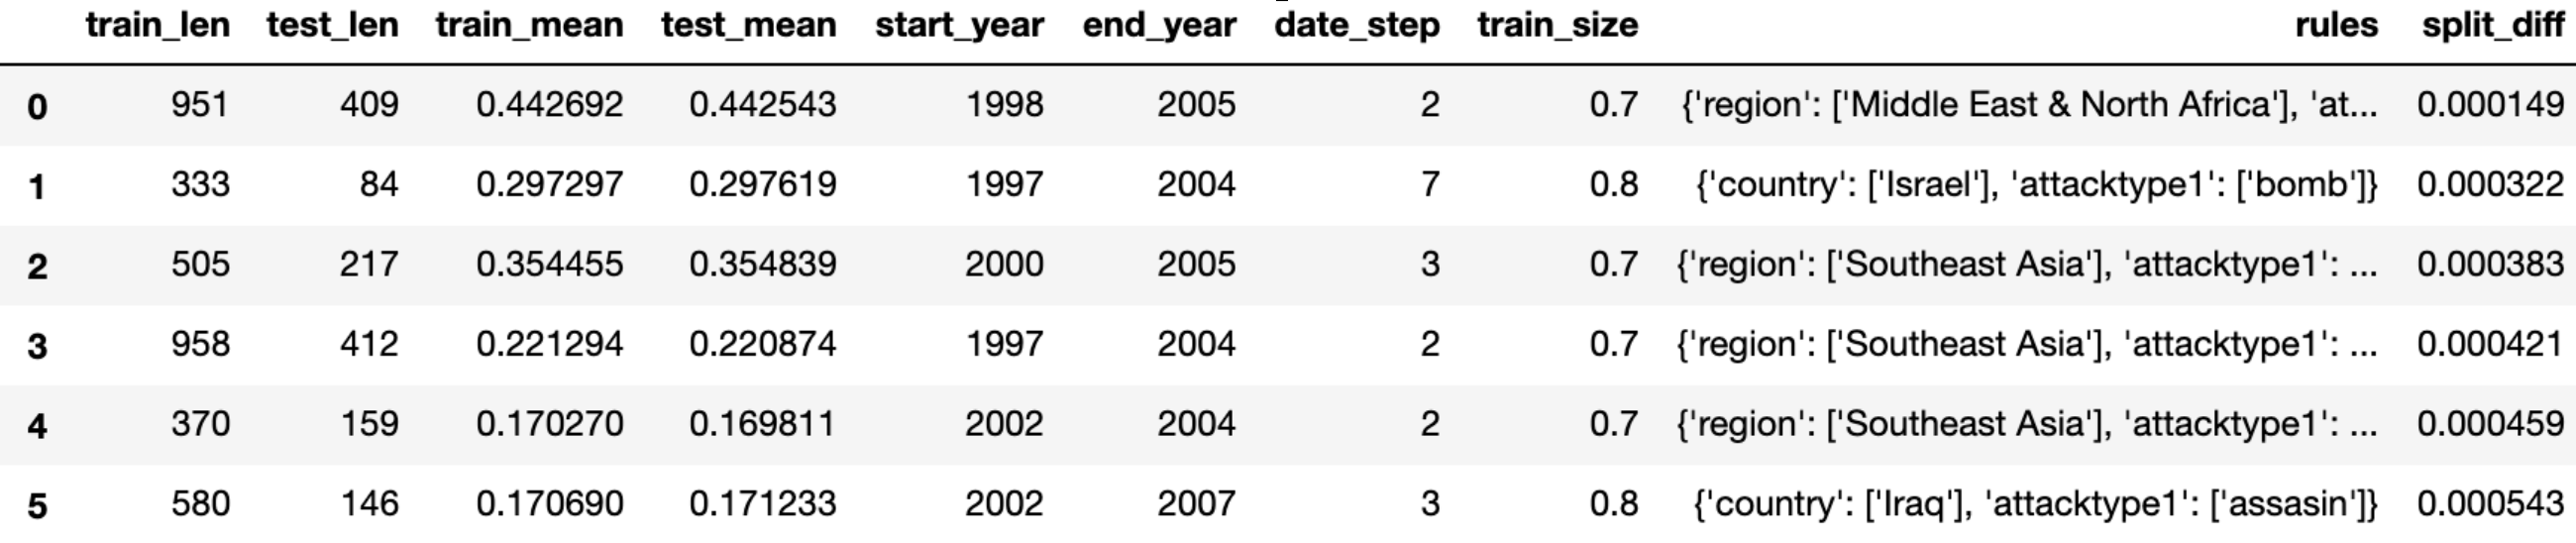
\includegraphics[width=\linewidth]{split_example.png}
%   \caption{Пример найденных разбиений для исходного набора данных}
%   \label{fig:split_example}
% \end{figure}

\subsubsection{Использование текстовых данных} \label{lda_topics}
% LDA model and document merging over agg period
В дополнение к существующим исходным признакам было решено использовать текстовые описания событий, а точнее соответствующие им вектора признаков, полученные с помощью модели Латентного размещения Дирихле (LDA) \cite{lda_orig}.
 
Модель Латентного размещения Дирихле представляет из себя статистическую модель, используемую в основном в задачах обработки текстов. Эта модель работает с документами, которые в свою очередь являются последовательностью термов (слов). Для заранее заданного числа скрытых (латентных) тем LDA позволяет построить два распределение: распределения тем по документам и распределения термов по темам. После того как модель обучена на $N$ документах для количества тем равного $K$ и количества различных термов равного $V$, мы получаем две матрицы весов $\theta \in \mathbf{R}^{N \times K}$ и $\phi \in \mathbf{R}^{K \times V}$, характеризующие параметры распределения Дирихле. Матрица $\theta$ отражает распределение тем по документам, а матрица $\phi$ -- распределение термов по темам.

Для получения значений скрытых тем новых документов необходимо их так же предобработать так же, как и тексты на которых производилось обучение, а затем, используя матрицу $phi$ получить значения скрытых тем из текстового содержания документа.

В рамках экспериментов алгоритм использования текстовых признаков с помощью модель Латентного размещения Дирихле выглядит следующим образом:
\begin{enumerate}
    \item Для каждого агрегационного периода получить единственный текстовый документ путем конкатенации (склеивания) всех текстовых описаний событий, входящих в период.
    \item Произвести классическую предобработку этих документов: удалить пунктуацию, нормализовать слов, удалить стоп-слова, ....
    \item Используя эти документы (точнее ту их часть, которая относится к тренировочной выборке) построить LDA-модель, т.е. построить распределение тематик по документам и распределение слов по тематикам для заданного количества тематик (в экспериментах количество тематик берется равным 10)
    \item Используя модель из предыдущего пункта получить 10 дополнительных признаков (соответствующих текстовым тематикам) для каждого агрегационного периода и использовать их вместе (с помощью конкатенации) с признаками, соответствующими скрытому представлению.
\end{enumerate}

Пример пяти тематик (их ключевых слов), выделенных с помощью LDA:
\begin{enumerate}
    \item incid bomb kill total relat
    \item claim respons group region kill
    \item group respons claim bomb injur
    \item incid target algerian take place
    \item algerian take place forc kill
\end{enumerate}

\begin{figure}
  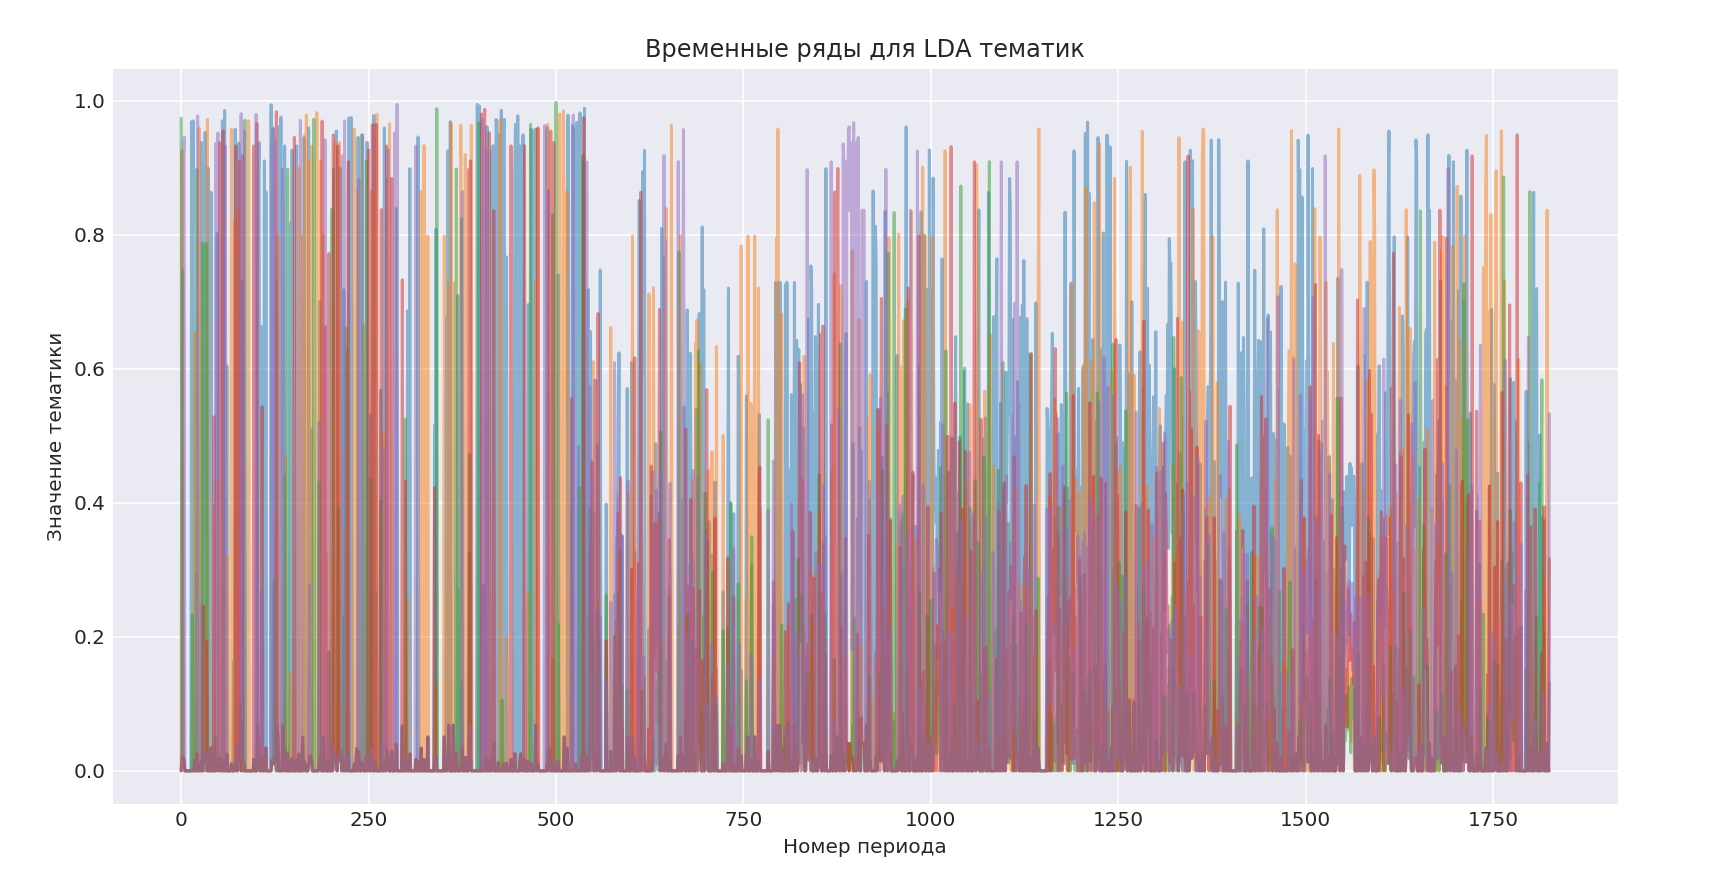
\includegraphics[width=\linewidth]{lda_example.png}
  \caption{Пример временных рядов для тематик LDA}
  \label{fig:lda_example}
\end{figure}

Пример соответствующих временных рядов можно увидеть на Рис. \ref{fig:lda_example}

\subsubsection{Результаты}
% Ниже приведены результаты для различных вариантов эксперимента.
Условия эксперимента:
\begin{enumerate}
    \item Год начала - 2002
    \item Год конца - 2008
    \item Длина агрегационного периода - 3 дня
    \item Тренировочная выборка: 70\%
    \item Целевые события: взрывы в Ираке (страна = Iraq, тип атаки = Bombing/Explosion)
\end{enumerate}
В рамках эксперимента были исследованы различные варианты представления событий -- с помощью NMF и с использованием автокодировщиков; количество тематик в экспериментах -- 10 и 50, так же вместе с тематиками были использованы дополнительные признаки AUX и REC.
В качестве моделей для прогнозирования были использованы классические модели классификации Logistic Regression (LogReg) и Random Forest Classifier (RFC), а так же нейронная сеть архитектуры LSTM.
Для задачи регрессии использовались модели Linear Regression (LinReg), Random Forest Regressor (RFR), а так же нейронная сеть архитектуры LSTM. Также варьировался размер окна исторических данных, которое мы принимали во внимание для построения прогноза. В текущем эксперименте были рассмотрены размеры окна равные 10 и 30.

В рамках экспериментов использовалась следующая архитектура сети LSTM: длина входной последовательности была равна 10 и 30 в зависимости от эксперимента и совпадала с размером окна исторических данных. Размерность скрытого слоя состояния LSTM-блока была равна размерности скрытого представления $k$ и принимала значения равные 10 и 50. При решении задачи прогнозирования вероятности события мы использовали функцию softmax для преобразования выхода сети в вероятности. В случае прогнозирования количества событий мы использовали линейную функцию активации. В процессе тренировки нейронной сети темп обучения был выбран равным $10^{-3}$, а количество эпох равным 50.

Обозначения:
\begin{itemize}
    \item  NMF\_N / AE\_N - использование тематик полученных с помощью NMF / Автокодировшика и с использованием N тематик
    \item + A - использование 2 дополнительных признаков (AUX), добавляющих авторегрессионную составляющую и описанных в \ref{train_process}
    \item + R - использование дополнительного признака, отвечающего за ошибку восстановления (реконструкции) в автокодировщике и описанного в \ref{train_process}
    %\item + text - использование 10 дополнительных тематик, описанных в \ref{lda_topics}
\end{itemize}

\subsubsection{Прогнозирование вероятности события}
Поскольку задача прогнозирования вероятности события сводится к задаче классификации и определения, произойдет событие или нет, для решения этой задачи были выбраны модели классификации.
В таблицах \ref{tab:clf-res-no-text} и \ref{tab:clf-res-text} представлены результаты решения задачи по метрике ROC AUC (чем меньше, тем лучше) для различных моделей и условий тестирования. Лучшие из обученных моделей смогли достигнуть ROC AUC $\approx$ 0.75-0.79. Лучшие результаты получали модели прогнозирования LSTM для всех трех вариантов извлечения этих тематик (матричная факторизация, автокодировщик, автокодировщик + ошибка восстановления). Также можно увидеть, что вспомогательные признаки (AUX) помогли моделям достигать более качественных результатов. Что касается размера окна (кол-ва исторических данных, использовавшихся для прогнозирования), то в среднем модели LSTM достаточно хорошо работали для размеров окна равных 10 и 30, в то время как классические модели (Random Forest Classifier, Logistic Regression) показывали более хорошие результаты на меньшем размере окна. Это может быть связанно с тем, что количество признаков при увеличении размера окна росло линейно и моделям было сложнее найти нужные паттерны в данных.
При использовании текстовых описаний модели LSTM показали как результатов, причем независимо от метода построения представления событий. Модели логистической регрессии и случайного леса на некоторых методах представления событий показали выигрыш по качеству с добавлением текстовых описаний, а на других стали работать немного хуже. Это, опять же, можно объяснить меньшей гибкостью линейных моделей и модели случайного леса.
\begin{center}
\begin{table}
 \begin{tabular}{||p{3.8cm}|p{1.5cm}|p{1.5cm}|p{1.5cm}|p{1.5cm}|p{1.5cm}|p{1.5cm}||} 
\hline
  & LSTM (L=10) & LSTM (L=30) & LogReg (L=10) & LogReg (L=30) & RFC (L=10) & RFC (L=30)\\ \hline\hline
AE\_10 & 0.616 & 0.641 & 0.439 & 0.417 & 0.484 & 0.509\\ \hline
AE\_10+A & 0.747 & 0.749 & 0.654 & 0.578 & 0.583 & 0.598\\ \hline
AE\_50 & 0.651 & 0.655 & 0.567 & 0.574 & 0.656 & 0.637\\ \hline
AE\_50+A & 0.743 & \textbf{0.752} & 0.655 & 0.552 & 0.658 & 0.578\\ \hline
AE\_10+R & 0.696 & 0.656 & 0.480 & 0.608 & 0.509 & 0.566\\ \hline
AE\_10+R+A & \textbf{0.764} & 0.744 & 0.653 & 0.572 & 0.609 & 0.615\\ \hline
AE\_50+R & 0.547 & 0.544 & 0.605 & 0.588 & 0.443 & 0.623\\ \hline
AE\_50+R+A & \textbf{0.761} & \textbf{0.760} & 0.655 & 0.551 & 0.659 & 0.606\\ \hline
NMF\_10 & 0.618 & 0.605 & 0.577 & 0.526 & 0.637 & 0.606\\ \hline
NMF\_10+A & 0.746 & 0.746 & 0.653 & 0.561 & 0.701 & 0.670\\ \hline
NMF\_50 & 0.691 & 0.711 & 0.537 & 0.446 & 0.650 & 0.533\\ \hline
NMF\_50+A & 0.740 & \textbf{0.783} & 0.658 & 0.580 & 0.638 & 0.671\\ \hline
 \end{tabular}
 \caption{\label{tab:clf-res-no-text} Результаты по метрике ROC AUC для задачи классификации без использования текста}
\end{table}
\end{center}

\begin{center}
\begin{table}
 \begin{tabular}{||p{3.8cm}|p{1.5cm}|p{1.5cm}|p{1.5cm}|p{1.5cm}|p{1.5cm}|p{1.5cm}||} 
\hline
& LSTM (L=10) & LSTM (L=30) & LogReg (L=10) & LogReg (L=30) & RFC (L=10) & RFC (L=30)\\ \hline\hline
AE\_10 & 0.597 & 0.657 & 0.505 & 0.563 & 0.679 & 0.361\\ \hline
AE\_10+A & \textbf{0.764} & 0.747 & 0.642 & 0.599 & 0.673 & 0.665\\ \hline
AE\_50 & 0.655 & 0.678 & 0.523 & 0.550 & 0.624 & 0.631\\ \hline
AE\_50+A & \textbf{0.752} & 0.745 & 0.645 & 0.493 & 0.681 & 0.614\\ \hline
AE\_10+R & 0.608 & 0.628 & 0.523 & 0.564 & 0.424 & 0.474\\ \hline
AE\_10+R+A & \textbf{0.795} & \textbf{0.758} & 0.642 & 0.576 & 0.644 & 0.619\\ \hline
AE\_50+R & 0.505 & 0.553 & 0.523 & 0.552 & 0.575 & 0.616\\ \hline
AE\_50+R+A & 0.736 & \textbf{0.759} & 0.644 & 0.523 & 0.674 & 0.504\\ \hline
NMF\_10 & 0.612 & 0.743 & 0.476 & 0.563 & 0.652 & 0.615\\ \hline
NMF\_10+A & 0.601 & \textbf{0.753} & 0.644 & 0.544 & 0.674 & 0.567\\ \hline
NMF\_50 & \textbf{0.776} & 0.688 & 0.484 & 0.547 & 0.575 & 0.498\\ \hline
NMF\_50+A & 0.741 & \textbf{0.753} & 0.645 & 0.569 & 0.688 & 0.625\\ \hline
 \end{tabular}
 \caption{\label{tab:clf-res-text} Результаты по метрике ROC AUC для задачи классификации с использованием текста}
\end{table}
\end{center}

\begin{figure}
  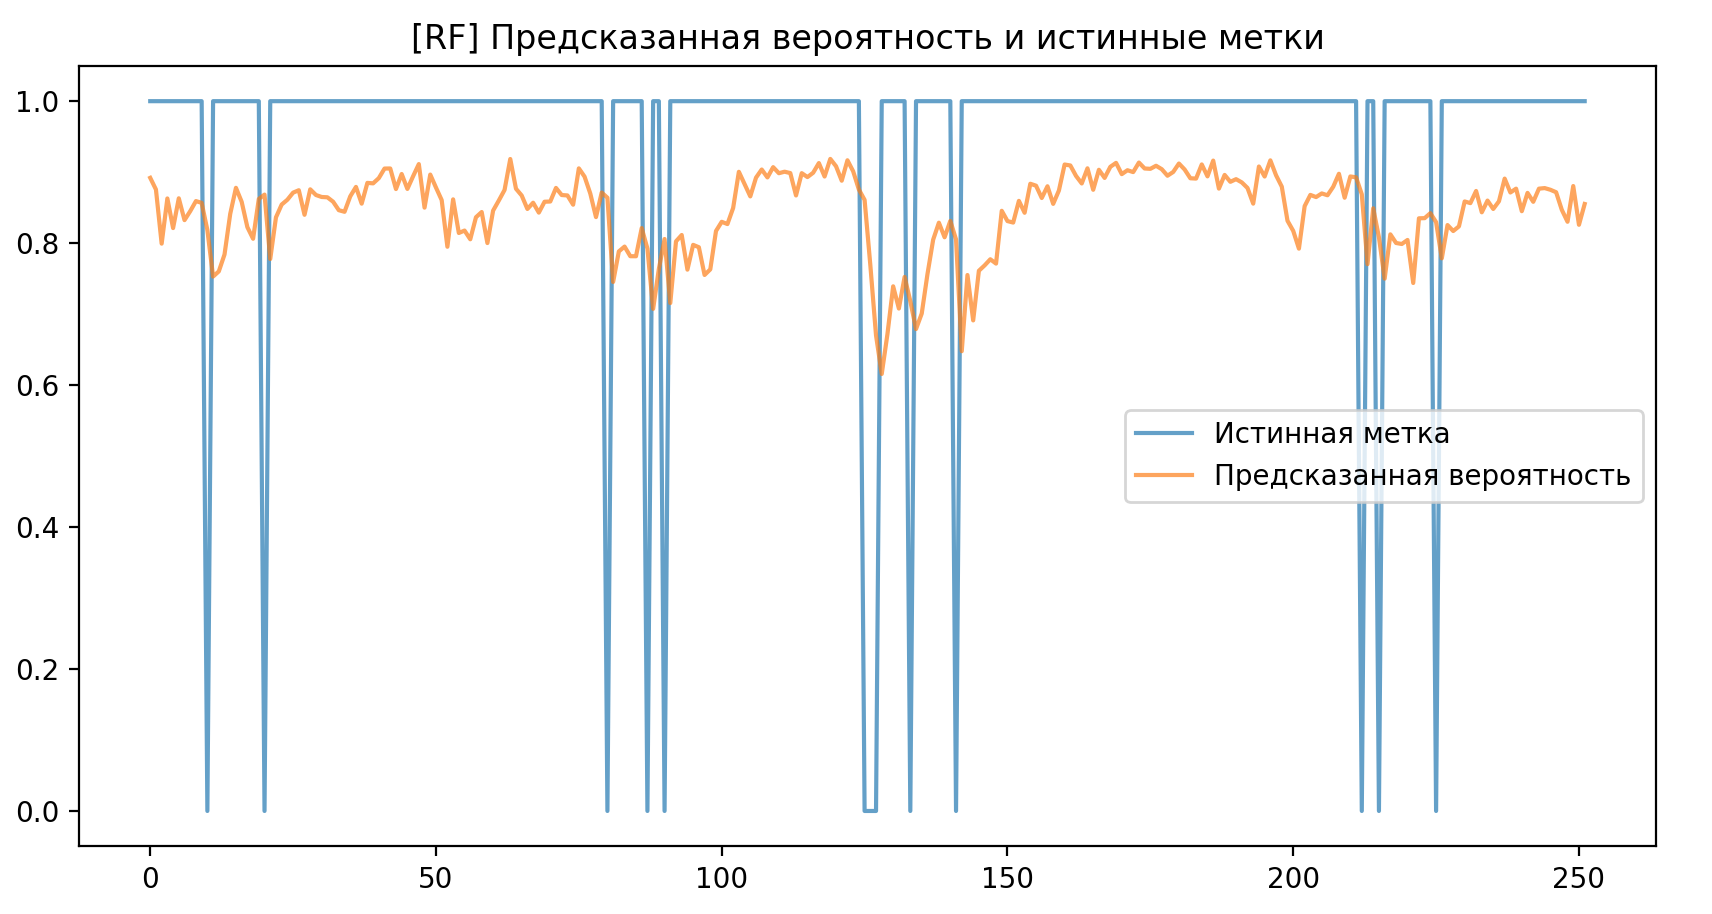
\includegraphics[width=\linewidth]{rf_clf_example.png}
  \caption{Пример работы модели классификации}
  \label{fig:rf_clf_example}
\end{figure}

\subsubsection{Прогнозирование количества событий}
Задача прогнозирования количества событий является задачей регрессии и может быть решена соответствующими моделями. В рамках экспериментов были рассмотрены модели линейной регрессии, случайного леса и нейросетевая модель архитектуры LSTM.
В таблицах \ref{tab:reg-res-no-text} и \ref{tab:reg-res} представлены результаты решения задачи регрессии по метрике MASE (чем меньше, тем лучше) для различных моделей и условий тестирования.

Исследовав распределение целевой переменной было решено попробовать предсказывать не количество $n$ событий, а величину $n' = log(1+n)$, восстанавливая затем $n$. Обозначим предсказанный логарифм как $y'$, а искомую величину за $y$. Тогда восстановить $y$ использую $y'$ можно следующим образом:
$$ y = e^{y' + \frac{\epsilon}{2}} - 1 $$
где $\epsilon$ - значение среднеквадратичной ошибки на специальной отложенной выборке.
Поскольку в этом случае требуется отложенная (валидационная) выборка, разбиение данных производится в пропорции 0.7 (тренировочная выборка) + 0.1 (валидационная) + 0.2 (тестовая). 

Лучше всех из регрессионных моделей себя показал случайный лес, стабильно достигая MASE = 0.9. Способ извлечения тематик, как оказалось, не играет решающей роли, как и количество интервалов, используемых для прогнозирования. Можно заметить, что дополнительные AUX-признаки значительно улучшают результаты, это вполне может быть вызвано тем, что они помогают модели случайного леса находить авторегрессионные зависимости, которые без этих дополнительных признаков найти было бы нетривиально. 
Какой-то сильной зависимости от использования или неиспользования текстовых признаков здесь обнаружить не удается, таким образом можно сделать вывод что решению задачи прогнозирования количества событий для рассмотренных моделей и методов построения представления использование текстовых признаков не помогает.
\begin{center}
\begin{table}
 \begin{tabular}{||p{3.8cm}|p{1.5cm}|p{1.5cm}|p{1.5cm}|p{1.5cm}|p{1.5cm}|p{1.5cm}||} 
\hline
& LSTM (L=10) & LSTM (L=30) & LinReg (L=10) & LinReg (L=30) & RFR (L=10) & RFR (L=30)\\ \hline\hline
AE\_10 & 1.218 & 1.204 & 1.119 & 1.191 & 1.241 & 1.265\\ \hline
AE\_10+A & 1.050 & 1.050 & \textbf{0.909} & 1.074 & \textbf{0.890} & \textbf{0.909}\\ \hline
AE\_10+R & 1.092 & 1.096 & 1.121 & 1.193 & 1.239 & 1.287\\ \hline
AE\_10+R+A & 1.054 & 1.072 & \textbf{0.911} & 1.102 & \textbf{0.886} & \textbf{0.910}\\ \hline
AE\_50 & 1.119 & 1.155 & 1.180 & 1.657 & 1.244 & 1.257\\ \hline
AE\_50+A & 1.084 & 1.055 & 1.632 & 1.616 & \textbf{0.883} & \textbf{0.904}\\ \hline
AE\_50+R & 1.040 & 1.039 & 1.209 & 1.580 & 1.243 & 1.278\\ \hline
AE\_50+R+A & 1.059 & 1.056 & 1.632 & 1.758 & \textbf{0.876} & \textbf{0.916}\\ \hline
NMF\_10 & 1.218 & 1.194 & 1.096 & 1.422 & 1.094 & 1.182\\ \hline
NMF\_10+A & 1.056 & 1.069 & \textbf{0.895} & 1.177 & \textbf{0.894} & \textbf{0.929}\\ \hline
NMF\_50 & 1.136 & 1.128 & 1.336 & 1.112 & 1.092 & 1.155\\ \hline
NMF\_50+A & 1.076 & 1.061 & 1.468 & 1.181 & \textbf{0.913} & \textbf{0.912}\\ \hline
  
\end{tabular}
\caption{\label{tab:reg-res-no-text} Результаты по метрике MASE для задачи регрессии без использования текста}
\end{table}
\end{center}

\begin{center}
\begin{table}
 \begin{tabular}{||p{3.8cm}|p{1.5cm}|p{1.5cm}|p{1.5cm}|p{1.5cm}|p{1.5cm}|p{1.5cm}||} 
\hline
& LSTM (L=10) & LSTM (L=30) & LinReg (L=10) & LinReg (L=30) & RFR (L=10) & RFR (L=30)\\ \hline\hline
AE\_10 & 1.104 & 1.151 & 1.292 & 2.151 & 1.295 & 1.323\\ \hline
AE\_10+A & 1.084 & 1.058 & 1.025 & 1.924 & \textbf{0.898} & \textbf{0.925}\\ \hline
AE\_10+R & 1.148 & 1.133 & 1.312 & 1.920 & 1.287 & 1.306\\ \hline
AE\_10+R+A & 1.047 & 1.067 & 1.029 & 1.745 & \textbf{0.896} & \textbf{0.929}\\ \hline
AE\_50 & 1.148 & 1.120 & 3.492 & 1.862 & 1.300 & 1.307\\ \hline
AE\_50+A & 1.046 & 1.068 & 3.082 & 1.810 & \textbf{0.899} & \textbf{0.918}\\ \hline
AE\_50+R & 1.124 & 1.136 & 2.840 & 1.967 & 1.305 & 1.307\\ \hline
AE\_50+R+A & 1.057 & 1.051 & 2.152 & 2.126 & \textbf{0.895} & \textbf{0.919}\\ \hline
NMF\_10 & 1.171 & 1.068 & 1.241 & 2.921 & 1.171 & 1.187\\ \hline
NMF\_10+A & 1.077 & 1.059 & \textbf{0.973} & 2.280 & \textbf{0.894} & \textbf{0.933}\\ \hline
NMF\_50 & 1.168 & 1.108 & 3.534 & 1.212 & 1.123 & 1.148\\ \hline
NMF\_50+A & 1.072 & 1.062 & 3.094 & 1.205 & \textbf{0.902} & \textbf{0.910}\\ \hline
\end{tabular}
\caption{\label{tab:reg-res} Результаты по метрике MASE для задачи регрессии c использованием текста}
\end{table}
\end{center}




\begin{figure}
  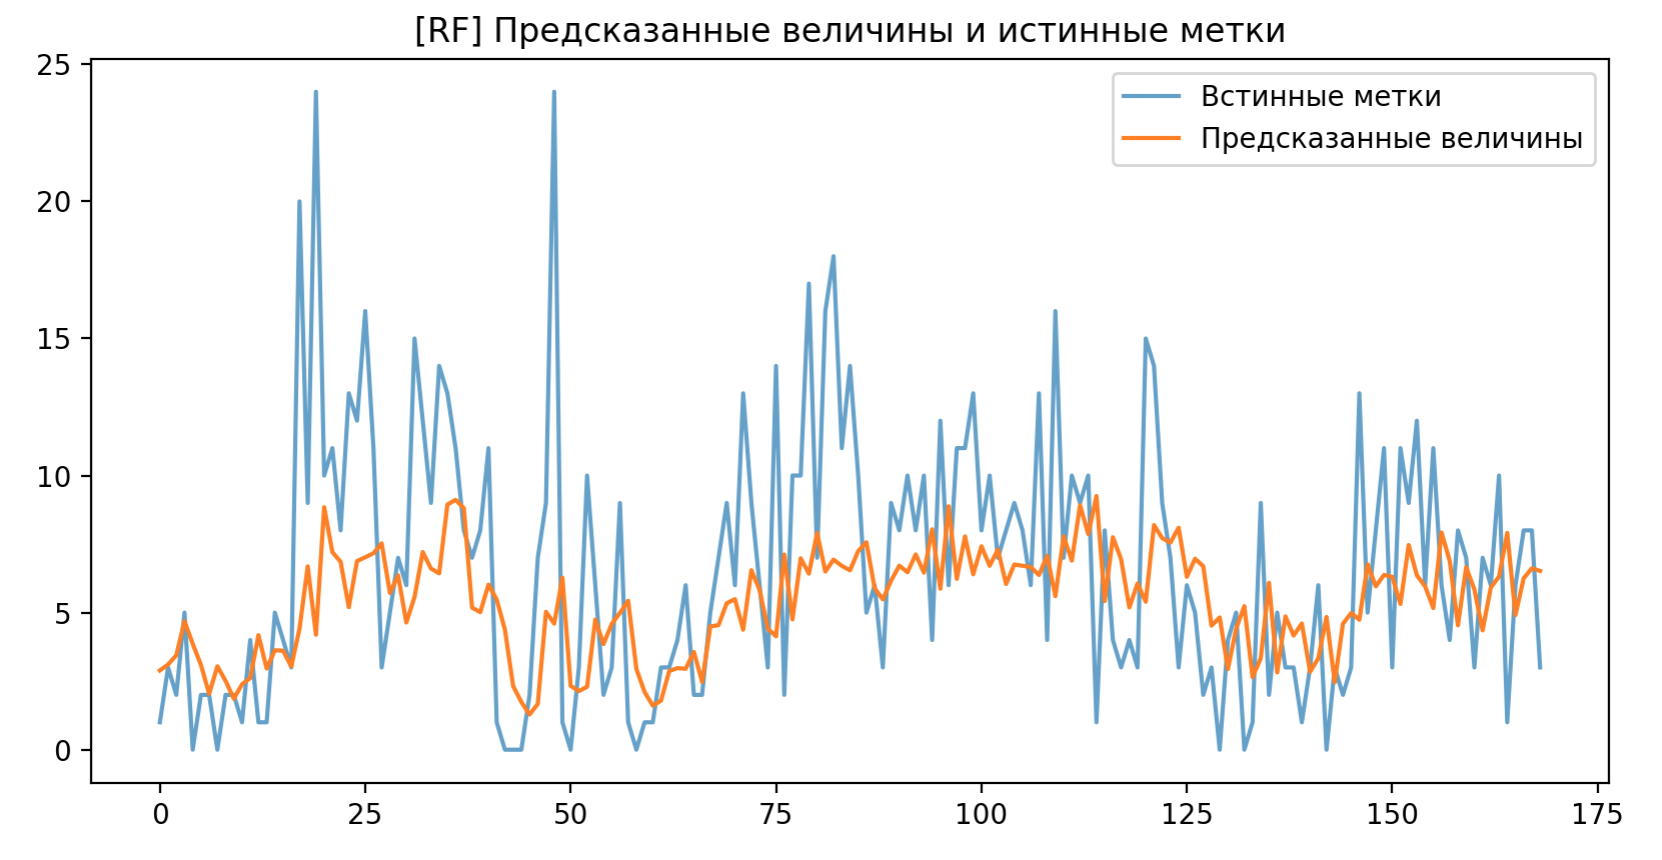
\includegraphics[width=\linewidth]{rf_reg_example.png}
  \caption{Пример работы модели регрессии}
  \label{fig:rf_reg_example}
\end{figure}

% \subsubsection{Регрессия логарифма целевой переменной}
% Исследовав распределение целевой переменной было решено попробовать предсказывать не количество $n$ событий, а величину $n' = log(1+n)$, восстанавливая затем $n$. Обозначим предсказанный логарифм как $y'$, а искомую величину за $y$. Тогда восстановить $y$ использую $y'$ можно следующим образом:
% $$ y = e^{y' + \frac{\epsilon}{2}} - 1 $$
% где $\epsilon$ - значение среднеквадратичной ошибки на специальной отложенной выборке.
% Поскольку в этом случае требуется отложенная (валидационная) выборка, разбиение данных производится в пропорции 0.7 (тренировочная выборка) + 0.1 (валидационная) + 0.2 (тестовая). 
% \par Ниже представлена метрика MASE (чем меньше, тем лучше) для различных моделей и условий тестирования. Метрика посчитана уже для восстановленных величин $y$.
% % description 
% % table
% \begin{center}
%  \begin{tabular}{||p{3.8cm}|p{1.5cm}|p{1.5cm}|p{1.5cm}|p{1.5cm}|p{1.5cm}|p{1.5cm}||} 
% \hline
%   & RFR (lag=10) & RFR (lag=30) &   LinReg (lag=10) & LinReg (lag=30) & LSTM (lag=10) & LSTM (lag=30)  \\ 
% \hline\hline
%  \hline
% \end{tabular}
% \end{center}
